\chapter{YOLO 类双目标检测模型的边缘兼容迁移方法}
\label{cha:method}

本章给出论文的核心方法。这里不把模型训练和板端运行分开处理，而是把 YOLO 类双目标检测模型从训练权重迁移到目标平台、再进入设备端执行的过程视为一条需要保持语义一致的系统链路。围绕 HongOU PI（Hi3516DV500）开发板和 YOLOv8n 模型，模型训练、ONNX 导出、OM 编译和板端验证被组织为连续流程，使 \textit{person} 与 \textit{ebike} 两类目标的输入、类别、边框、阈值和运行状态都有可检查的约束。

\section{总体技术路线}

图 \ref{fig:migration_pipeline} 给出了方法总体流程。训练阶段得到的 YOLO 双目标检测权重先经过类别数与检测头适配检查，再导出为 ONNX 中间表示；随后通过 ATC 编译得到边缘设备可执行的 OM 模型；进入板端后，系统完成 NPU 推理、输出解析、阈值筛选和后处理，并与统一实验协议下的结果进行一致性分析。

\begin{figure}[htbp]
    \centering
    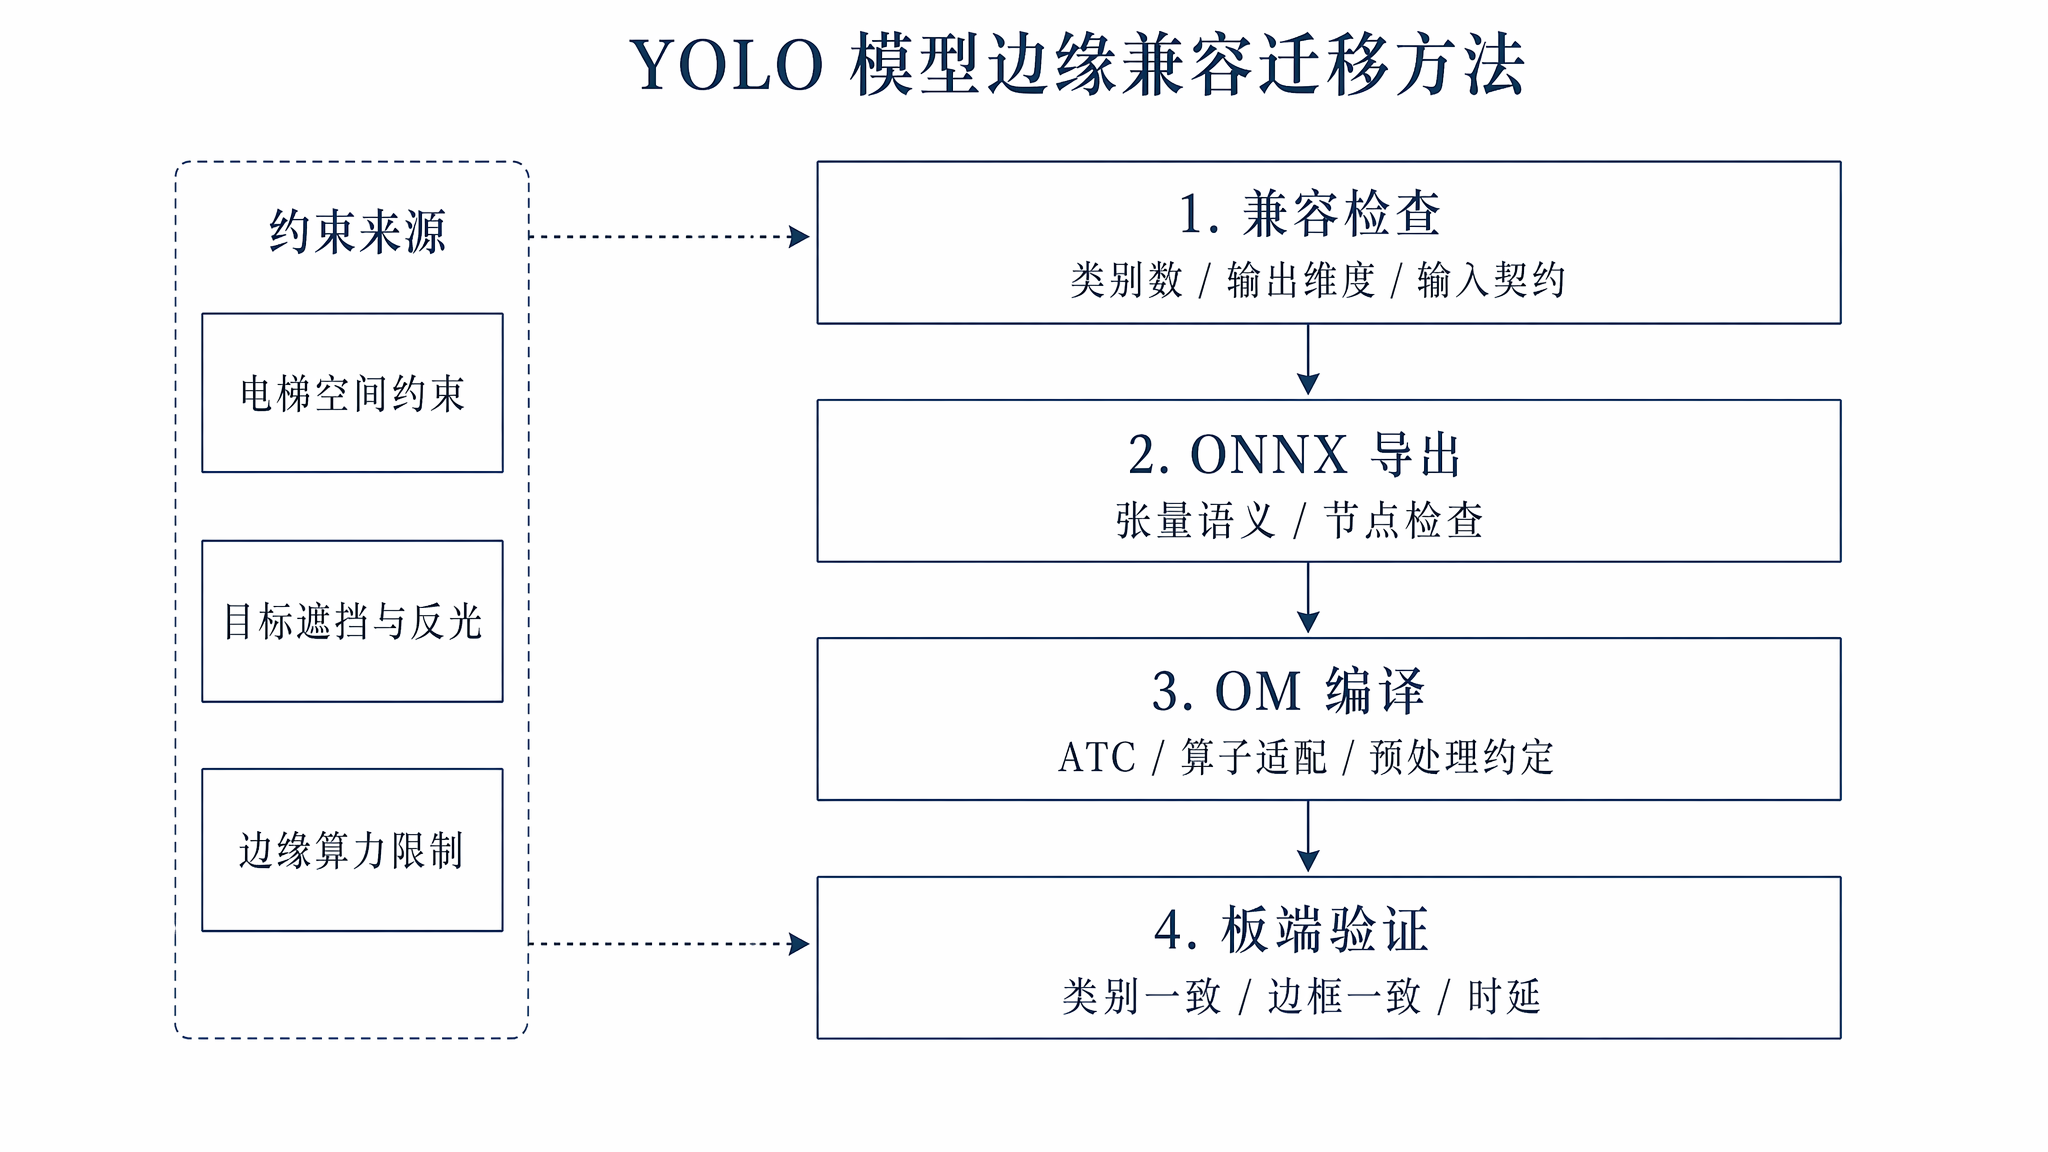
\includegraphics[width=\textwidth]{image/fig4-migration-method.png}
    \caption{YOLO 双目标检测模型的边缘兼容迁移流程}
    \label{fig:migration_pipeline}
\end{figure}

这条流程的关键不只在模型文件能否生成。模型层需要保证检测头输出与双目标任务一致，避免类别数或类别顺序错误；格式层要检查 PyTorch、ONNX 和 OM 之间的输入输出张量语义是否一致；应用层则要让板端后处理逻辑与训练框架中的统计口径保持可比较。YOLOv5、YOLOv8 等 YOLO 类检测器在部署时都会涉及输入预处理、类别维度、检测头输出、候选框解码、置信度筛选和 NMS 等环节，因此本章按照这些共性接口组织迁移方法，并在 YOLOv8n 板端链路中展开具体实现与实验分析。只有这些约束同时成立，边缘设备端的检测指标才有解释意义。

迁移检查在论文中分为语义、数值和运行三个层次。语义检查包括类别数量、类别顺序和输出张量维度；数值检查包括边框坐标、置信度范围和 NMS 后检测数量；运行检查包括模型加载、推理成功率、验证链路端到端耗时和关键分段耗时。这样的顺序先确认基础语义，再讨论 mAP 等检测指标，同时把 batch 外围链路耗时与模型执行阶段耗时分开解释，避免把不同运行口径混在一起。

\section{YOLOv8n 场景化训练与验证性能}

进入板端部署前，双目标检测模型先在 Ultralytics YOLOv8n 框架下完成场景化训练。训练环境为 x86\_64 工作站，主要硬件包括 Intel Xeon Gold 6226R CPU、约 125 GiB 系统内存和 4 张 NVIDIA GeForce RTX 3090 GPU；本次训练使用第 0 号 GPU。训练任务使用 \textit{person} 与 \textit{ebike} 两类标注，输入尺寸为 $640 \times 640$，batch size 为 16，训练 100 个 epoch，并以 COCO 预训练 YOLOv8n 权重作为初始化。该 YOLOv8n 模型对应后续 ONNX 导出、ATC 编译和 OM 板端部署的源权重，训练阶段验证结果也就成为分析板端指标回退幅度的参照。

图 \ref{fig:chap03_training_results} 给出了训练过程中的损失和验证集指标曲线。可以看到，训练后期 box loss、classification loss 和 DFL loss 继续保持下降或趋稳，验证集 precision、recall 和 mAP 指标整体维持在较高水平，未出现明显的训练发散现象。

\begin{figure}[htbp]
    \centering
    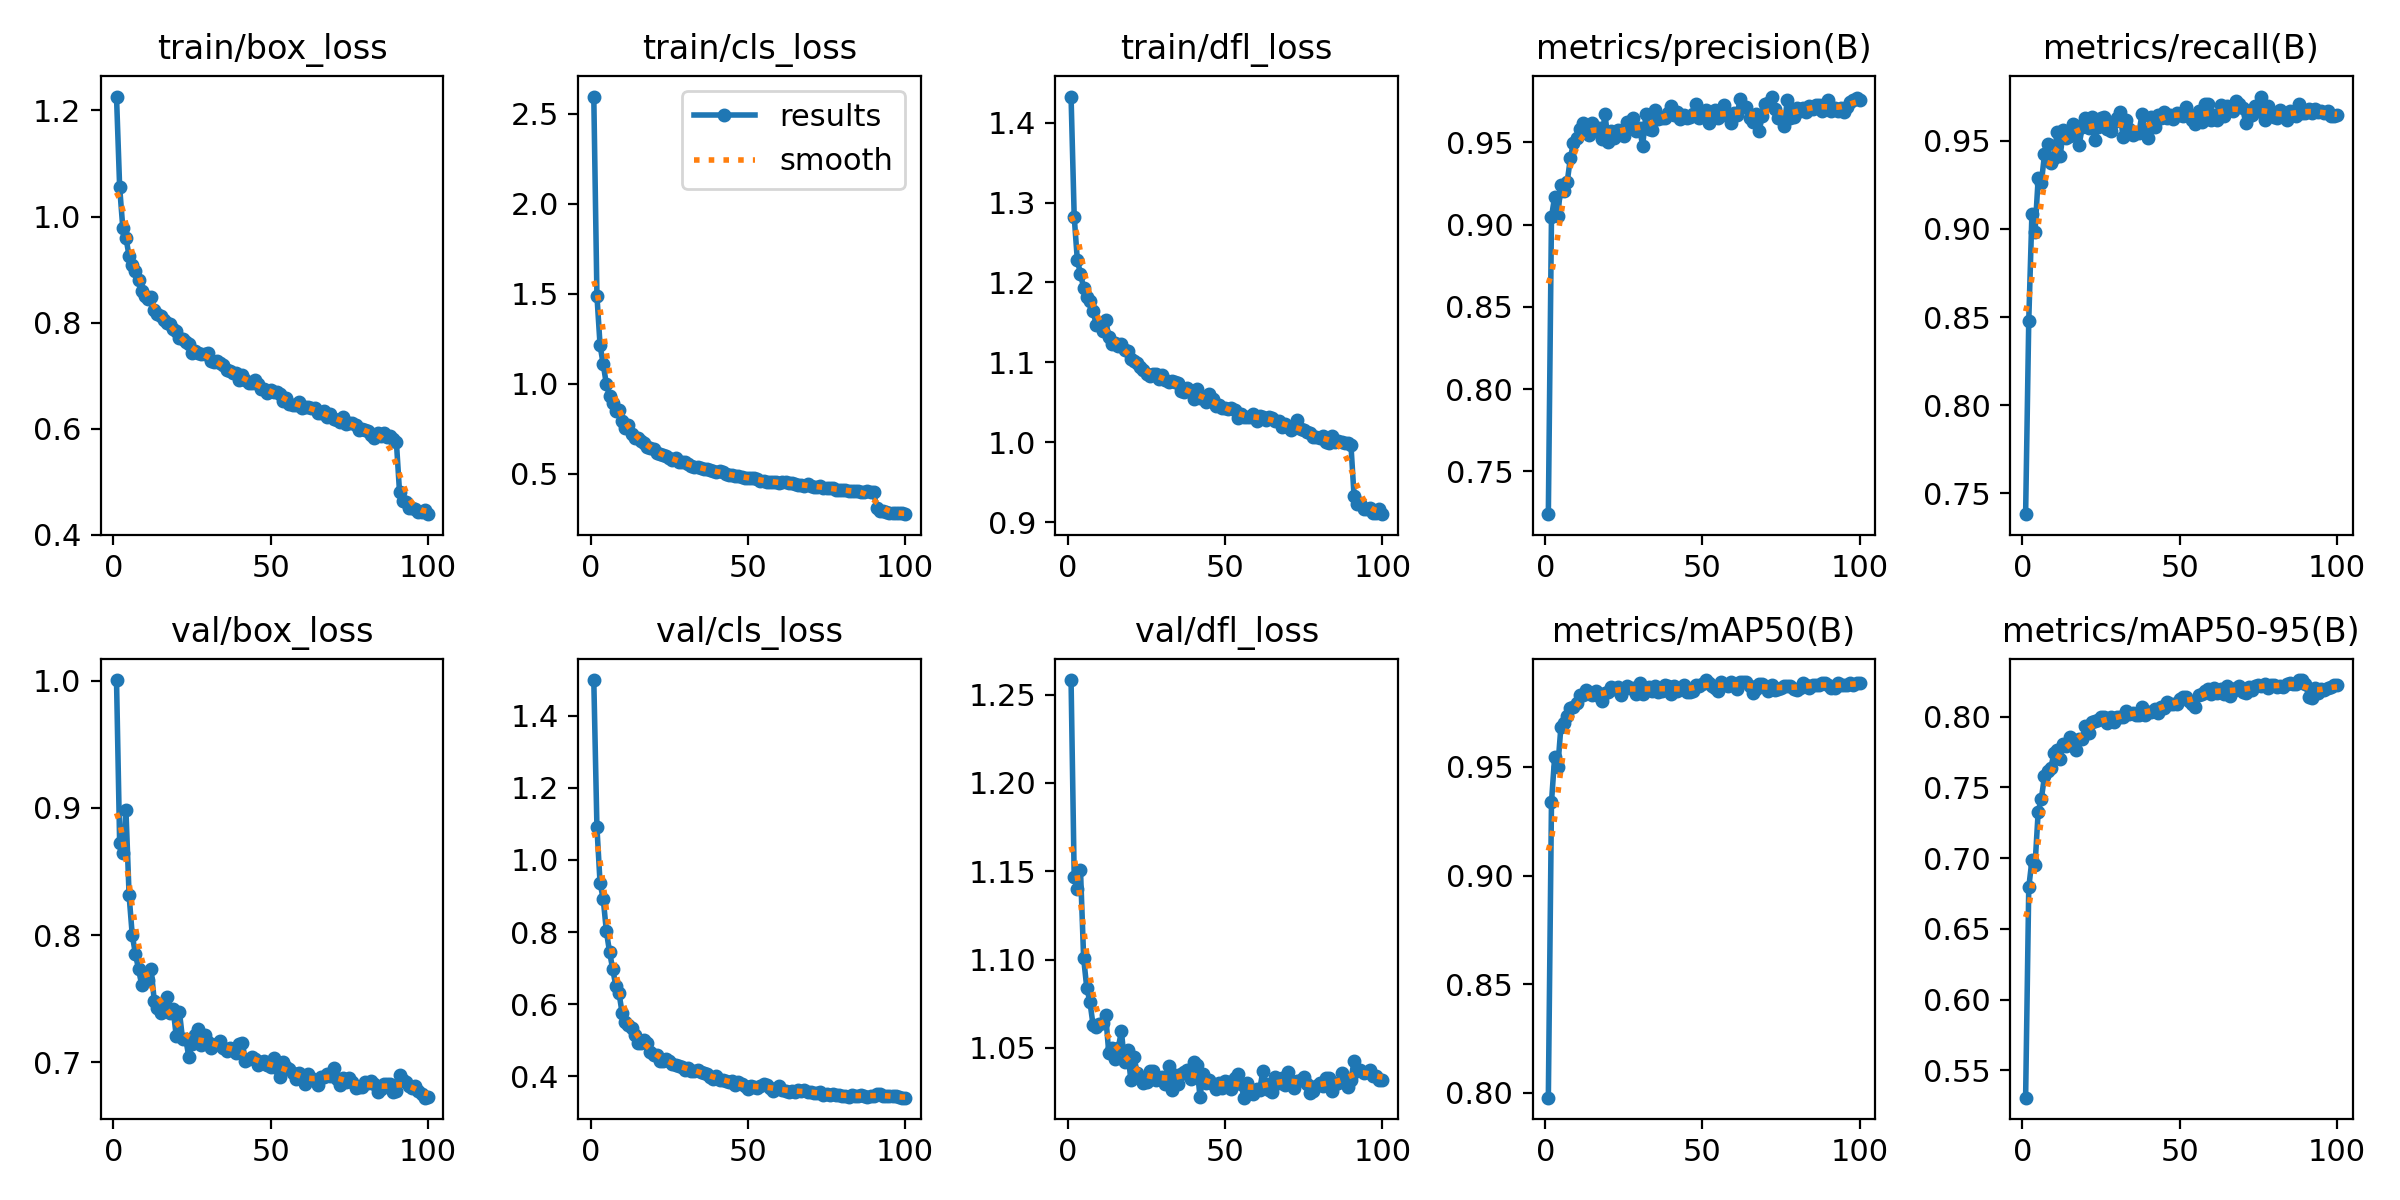
\includegraphics[width=\textwidth]{image/generated/fig_chap03_training_results.png}
    \caption{YOLOv8n 场景化训练曲线}
    \label{fig:chap03_training_results}
\end{figure}

第 100 个 epoch 的验证集 precision 为 0.9756，recall 为 0.96469，mAP@0.5 为 0.98832，mAP@0.5:0.95 为 0.82203。从这个结果看，场景化训练后的 YOLOv8n 模型在训练阶段已经具备较强的双目标检测能力。第五章进一步将训练阶段验证结果与 Hi3516DV500 板端 FP16/OM 结果对照，用于解释部署后指标的保留程度和回退幅度。

\begin{figure}[htbp]
    \centering
    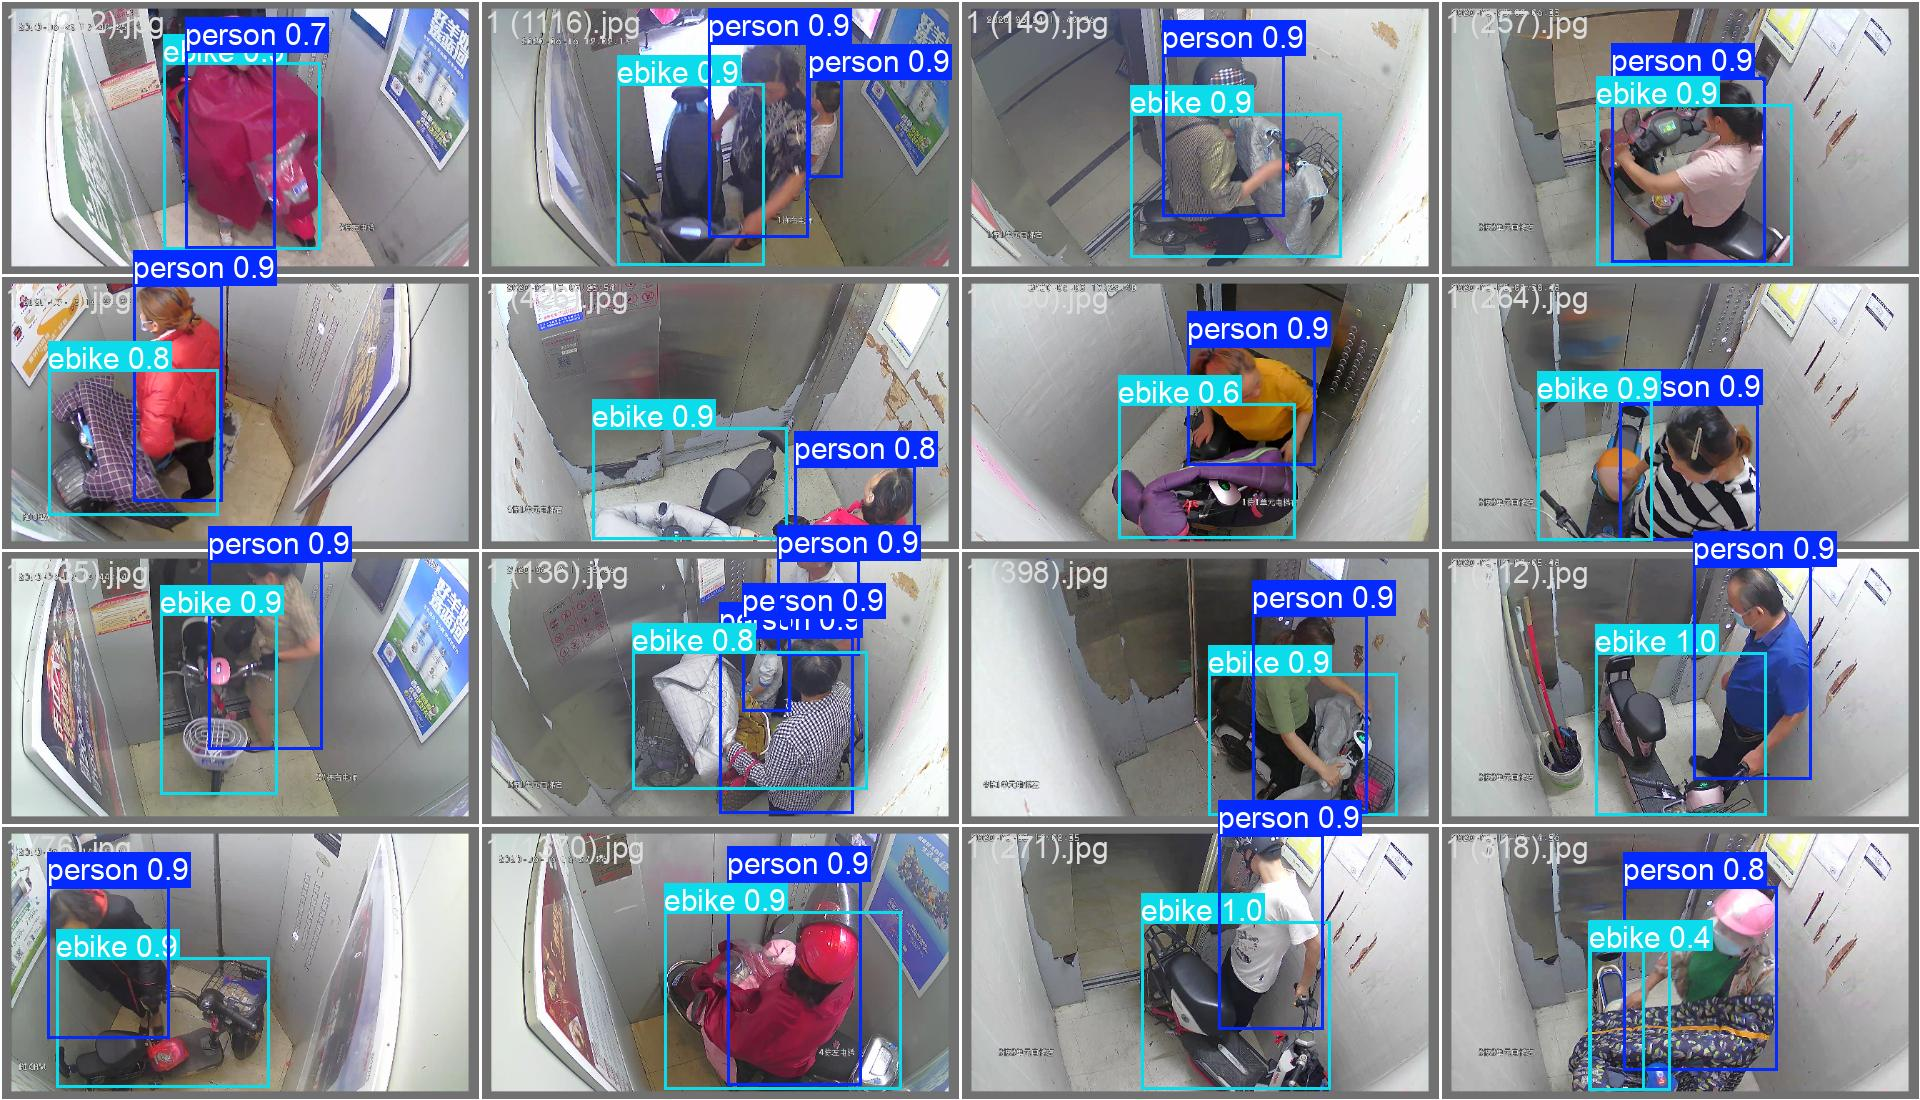
\includegraphics[width=\textwidth]{image/generated/fig_chap03_training_val_predictions.jpg}
    \caption{YOLOv8n 场景化训练模型验证集预测示例}
    \label{fig:chap03_training_val_predictions}
\end{figure}

图 \ref{fig:chap03_training_val_predictions} 展示了训练阶段模型在验证集上的预测输出。该图来自 YOLOv8n 训练流程保存的验证预测网格，用于直观说明模型已经能够在电梯视角下同时输出 \textit{person} 与 \textit{ebike} 检测框；训练阶段能力的定量判断仍以验证集 precision、recall 和 mAP 指标为依据。

\section{迁移约束与一致性检查}

迁移链路在本文中被抽象为接口契约。这里的契约不是额外算法模块，而是贯穿训练、导出、编译和板端运行的一组约束，用来把容易隐含在代码和配置中的输入、类别、输出、后处理和运行时假设显式化。对于 YOLO 类检测器而言，这些契约分别落在输入图像语义、类别维度、检测头张量、候选框解码、置信度阈值、NMS 策略和板端运行状态等环节。只有这些约束在各阶段保持一致，板端 precision、recall、F1 和 mAP@0.5 才能对应到真实检测行为。

输入契约约束输入尺寸、颜色通道、归一化、缩放与填充方式。电梯图像常包含强反光和大面积背景结构，若训练阶段和板端的缩放、填充或颜色通道处理不一致，模型对局部电动车结构的响应会发生变化，进而表现为分数漂移或小目标漏检。因此，输入契约要求训练配置、ONNX 输入形状、OM 模型输入和板端预处理路径采用一致的图像语义。

类别契约约束类别数量、类别顺序和标签名称。论文采用 \textit{person} 与 \textit{ebike} 两类标签，类别集合较小，但类别解释必须在训练配置、导出模型、板端标签表和后处理代码中完全一致。若类别维度读取或标签顺序发生错位，检测框位置即使正确，报警语义也会失效。

输出契约约束检测头张量维度、坐标格式和置信度含义。训练框架通常自动完成坐标解码和结果封装，而板端程序需要显式读取输出张量并解释其维度。如果坐标中心点、宽高、左上右下角或置信度分数组合方式被错误理解，最终结果会表现为边框漂移、类别分数异常或检测数量变化。

后处理契约约束置信度阈值、NMS 阈值和类别处理方式。电梯场景中的反光、门框和局部可见电动车会生成接近阈值的候选框，阈值和 NMS 的小幅变化可能改变最终安全输出。因此，后处理契约要求训练阶段统计脚本和板端应用层在阈值含义、NMS 输入、类别过滤和电动车清理策略上保持可比较。

运行契约约束模型文件、板端二进制、运行模式、成功样本数、失败样本数、端到端处理耗时和分段计时。该契约用于区分模型执行阶段、单帧处理路径和 batch 验证链路，避免把外围链路耗时误解为 OM/NPU 模型执行耗时，也避免在样本未处理完时报告全量验证结论。

为了让契约不只停留在概念层面，迁移链路采用逐项检查方式。ONNX 导出后检查输入尺寸和输出张量形状是否符合双目标检测设置；OM 编译后检查板端程序读取的输出数量和张量维度是否与导出阶段一致；运行验证集时，再看成功样本数、分类别预测数和分类别 TP/FP/FN 是否处于合理范围。若某一项出现异常，优先回到对应契约定位问题，而不是直接调整阈值掩盖错误。

分阶段验证策略强调每一阶段只解决少数关键问题。训练阶段主要看模型是否具备基础检测能力，并保留权重文件与验证集指标；导出阶段检查输入输出形状和类别维度是否保留；编译阶段关注 OM 模型能否生成以及算子是否兼容；板端阶段再检查推理成功率、后处理结果、检测框、分类别指标和运行时信息。这样做可以降低排错复杂度，使板端结果异常时能够回溯问题来源。

下面对五类约束的关键一致性环节分别说明。

\subsection{输入预处理对齐}

输入预处理对齐要求训练阶段、导出阶段和板端使用相同的输入尺寸与图像变换语义。对于固定视角电梯场景，目标尺度分布相对集中，但近景人体和局部电动车会使边缘区域信息非常重要。因此，预处理不应仅追求图像尺寸匹配，还需要保证缩放比例、填充区域和坐标还原方式能够被后处理正确反推。

\subsection{类别语义对齐}

类别语义对齐是双目标任务迁移中最基础的契约。本文包含 \textit{person} 与 \textit{ebike} 两个类别，类别数较少反而要求类别解释更加清晰。训练配置、导出模型、板端标签表和后处理代码必须使用相同类别顺序；否则，即使检测框位置正确，最终报警语义也可能被反转。

在实验解释中，分类别 TP、FP、FN 统计也被用作类别契约的外部检查。若板端程序把类别维度读取错误，\textit{person} 与 \textit{ebike} 的预测数量、召回率和 mAP@0.5 会出现与场景经验明显不符的异常。因此，分类别指标不仅衡量检测性能，也用于判断迁移后的语义解释是否成立。

\subsection{输出张量语义对齐}

输出张量语义对齐要求板端程序明确知道 YOLO 检测头输出中每一维的含义。本文关注的双目标检测只有两个类别，但这反而要求类别维度更清晰：如果板端按错误类别数读取张量，类别分数的位置会发生偏移；如果按错误坐标格式解释边框，IoU 指标会下降。因此，输出张量检查是迁移流程中的必要步骤，它决定后续实验结果能否对应到真实检测行为。

\subsection{后处理一致性}

后处理一致性包括置信度筛选和 NMS 两部分。置信度阈值决定候选框进入最终结果的机会，NMS 决定重叠候选框的保留关系。电梯场景中的反光、门口结构和局部可见目标会产生大量边界候选框，因此阈值口径会直接影响安全输出。实验章通过阈值敏感性分析观察不同置信度阈值下 precision、recall、F1 和分类别召回率的变化。

后处理既可以在模型图中完成，也可以在应用层完成。若后处理前移到模型图中，板端应用更简单，但阈值和 NMS 策略调整不够灵活；若后处理保留在应用层，便于针对安全场景调整阈值，但应用层必须正确实现坐标解码和候选框抑制。本文选择应用层后处理思路，并通过契约方式约束其输入、阈值和输出含义。

\subsection{运行时可靠性}

运行时可靠性要求设备端不仅能够加载 OM 模型，还能够完成验证集推理并记录成功样本数、失败样本数、验证链路端到端耗时和关键分段耗时。对于安全视觉系统，单张图像推理成功不足以说明系统可用；只有在统一数据集上可靠执行，并能说明耗时指标属于哪一段链路，设备端结果才具备分析意义。

运行时可靠性还需要关注异常样本处理。若某些图像推理失败，实验报告应区分模型检测错误和运行失败；若大量样本触发兜底路径或超时，端到端耗时也需要与成功样本数一起解释。结果章会报告成功样本数、失败样本数、batch 图像验证链路平均单图处理耗时和分段计时结果，使精度指标能够与板端运行状态共同解释。

\section{一致性分析方法}

本文从类别语义、边框解释、阈值行为和运行时状态四个角度分析迁移后一致性。类别语义检查不同阶段是否输出相同类别含义；边框解释关注坐标还原、IoU 衡量和定位漂移设计；阈值行为用于观察置信度阈值变化对 precision、recall 和 F1 的影响；运行时状态则记录成功样本数、失败样本数、端到端处理耗时和分段计时。这些内容共同构成本文的分析框架。

具体到方法层面，类别一致性依靠类别顺序和分类别 TP/FP/FN 判断 \textit{person} 与 \textit{ebike} 语义是否可靠；边框解释借助 IoU、边框漂移设计和 NMS 后数量判断定位变化是否影响检测结果；阈值口径通过多阈值 P/R/F1 与 \textit{ebike} recall 判断安全输出是否依赖单一参数；运行时可靠性则通过成功样本数、失败样本数、端到端耗时和分段计时判断板端验证是否执行完毕，并区分 batch 外围链路与模型执行阶段。

跨阶段逐样本匹配是迁移后一致性分析的扩展形式。实验章重点报告板端验证集结果、分类别结果、阈值敏感性后验重算、NMS 敏感性、后处理消融、视频输出状态和分段计时结果；PyTorch、ONNX、OM 和板端四阶段的逐样本匹配可用于进一步细化分析类别、坐标和分数在迁移链路中的变化。这样的处理使实验结论与证据范围保持对应。

样本级匹配的基本思路是：对于同一张输入图像，先按类别过滤候选框，再按 IoU 从高到低匹配同一目标，并比较不同阶段的类别、坐标和分数差异。若类别一致但 IoU 明显下降，主要问题可能来自坐标还原或 NMS；若 IoU 接近但类别不同，问题更可能来自类别顺序或输出维度解释；若同一阶段检测数量明显变化，则需要检查阈值和候选框抑制逻辑。该方法使跨阶段一致性从抽象概念转化为可执行的比较过程。

当结果出现异常时，本文先判断异常表现属于类别、边框、阈值还是运行状态，再回到对应契约检查。若类别大量错位，优先检查类别顺序和输出张量维度；若边框整体偏移，优先检查缩放、填充和坐标解释；若检测数量突变，优先检查 conf、NMS 和类别清理策略；若时延异常升高，优先检查板端执行路径、输入输出复制和资源状态。这种排查顺序把部署问题转化为可定位的技术项，便于复用。

\section{本章小结}

本章整理了面向目标平台约束的 YOLO 类双目标检测模型兼容迁移流程。流程围绕迁移约束展开，把输入预处理、类别配置、输出张量、后处理参数和运行状态纳入同一检查框架。相较于单纯报告模型精度，论文更关注模型进入板端后的行为能否解释、结果能否追溯。
